\chapter{[Google] ELECTRA: Pre-training Text Encoders as Discriminators Rather Than Generators}

\textbf{Reference:}~\url{https://arxiv.org/abs/2003.10555}

\textbf{Keywords:} language models, bert

\section*{Какую задачу решают авторы?}

Обучение больших языковых моделей (\textit{Language Models - LMs}) (BERT, XLM, GPT) чаще всего могут себе позволить лишь большие компании, так как это требует большого количества вычислительных ресурсов и времени.

В связи с этим, все большую популярность набирают исследования нацеленные на то чтобы сделать процесс обучения подобных моделей более эффективным, то есть более быстрым и дешевым. \\

Как правило, для предобучения LM используют задачу \textit{Masked language modeling (MLM)}:
\begin{itemize}
    \item В исходном тексте случайным образом заменяют часть токенов (чаще всего $15\%$) на специальный токен [MASK]
    \item Модель обучают корректно предсказывать маскированные токены
\end{itemize}

То есть в некотором смысле, для обучения модели используется только $15\%$ данных, что не очень эффективно. \\

В рамках данной работы, авторы предлагают по новому взглянуть на задачу для предобучения моделей, что позволяет обучать модели не только используя меньше ресурсов, но и получая при этом лучшие результаты на популярных бенчмарках (ускорение примерно в 30 раз).

\section*{Как решают}

Предложенный способ сильно напоминает процесс обучения GANов: модель \textit{генератор} обучается, решая задачу MLM, и заменяет часть токенов в исходном предложении на похожие, а модель \textit{дискриминатор} учится отличать оригинальные токены от сгенерированных (см. Рисунок~\ref{fig:electra}). Модели обучаются \textit{одновременно}.

\begin{figure}[ht]
  \centering
  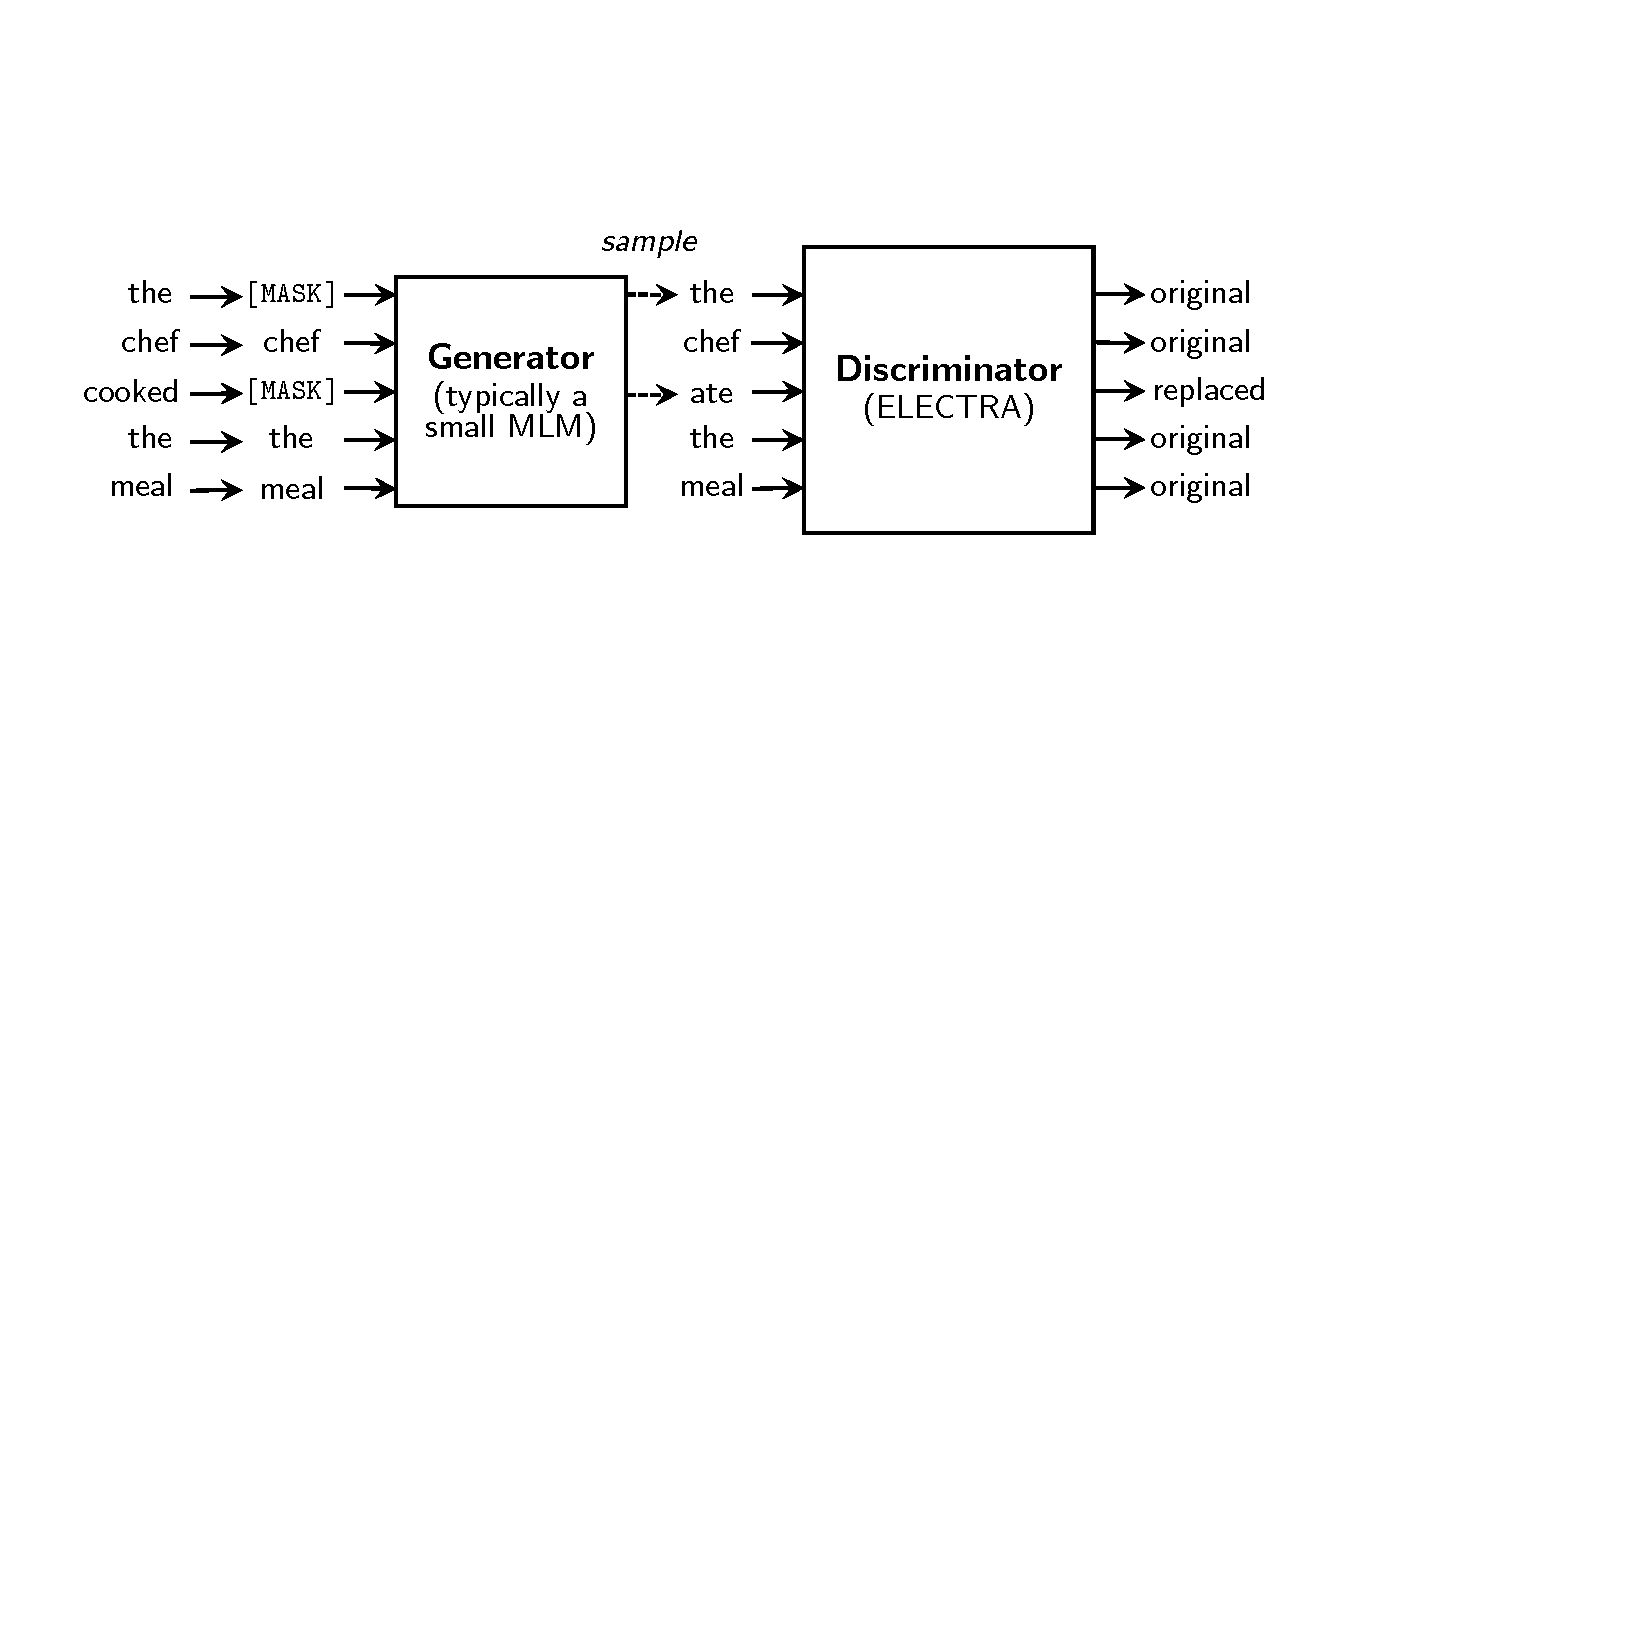
\includegraphics[width=0.8\linewidth]{figures/electra.pdf}
  \caption{}
  \label{fig:electra}
\end{figure}

Но в отличии от GANов генератор оптимизирует не \textit{adversarial loss}, а \textit{maximum likelihood}. 
После обучения моделей, генератор отбрасывается, а дискриминатор и есть итоговая обученная языковая модель. 
Так как предложенный фрэймвор не зависит от модели, в качестве архитектуры авторы выбрали BERT. \\

На первый взгляд кажется, что раз нужно обучать две модели, то обучение не должно стать быстрее. 
Но тут важную роль играет то, что для обучения дискриминатора используется весь исходный текст, а не только малая его часть.

Кроме того, авторы предлагают несколько практически трюков, которые позволяют добиться лучших результатов:
\begin{itemize}
    \item Для ускорения сходимости можно \textit{связать} параметры генератора и дискриминатора
    \item Даже если использовать в качестве генератора и дискриминатора разные модели, можно связать параметры эмбеддингов токенов
\end{itemize}

\section*{Мое мнение}

Работа в лишний раз подтверждает то, что важна не только архитектура модели, но и то как обучать модель.